\documentclass[11pt,a4paper]{article}
\usepackage{tla}\notla
\usepackage{isabelle,isabellesym}
\usepackage{amssymb}
\usepackage{graphicx}

% this should be the last package used
\usepackage{pdfsetup}

% urls in roman style, theory text in math-similar italics
\urlstyle{rm}
\isabellestyle{it}

\begin{document}

\title{Proving the Correctness of Disk Paxos in Isabelle/HOL}
\author{Mauro Jaskelioff\and Stephan Merz}
\maketitle

\begin{abstract}
  Disk Paxos~\cite{Gafni00disk} is an algorithm for building arbitrary
  fault-tolerant distributed systems. The specification of Disk Paxos
  has been proved correct informally and tested using the TLC model
  checker, but up to now, it has never been fully formally verified.
  In this work we have formally verified its correctness using the
  Isabelle theorem prover and the HOL logic
  system~\cite{Nipkow-Paulson-Wenzel:2002}, showing that Isabelle is a
  practical tool for verifying properties of TLA$^{+}$ specifications.
\end{abstract}

\tableofcontents

%%% The body of the paper

\section{Introduction}

Algorithms for fault-tolerant distributed systems were first
introduced to implement critical systems. Nevertheless, what good is
such an algorithm if it has a design error? We need some kind of
guarantee that the algorithm does not have a faulty design. Formal
verification of its specification is one such guarantee.

Disk Paxos~\cite{Gafni00disk} is an algorithm for building arbitrary
fault-tolerant distributed systems, that, due to its complexity, is
difficult to reason about. It has been proved correct informally, and
tested using the TLC model checker~\cite{LamportTLA:2002}. The
informal proof is rigorous but, as it is always the case with large
informal proofs, it is easy to overlook details. Thus, one of the
motivations of this work is to see if such a rigorous proof can be
formalized in a contemporary theorem prover.

In \cite{Pacheco-reasoning} part of the correctness proof (invariance
of \tla $HInv1$ and $HInv3$) \notla was verified using the theorem
prover ACL2~\cite{ACLBook}. An implicit assumption of this formalization is
that all sets are finite, thus overlooking the fact that there is a
missing conjunct in the Disk Paxos invariant 
(see Section \ref{sec:Structure-of-the}).

We set the goal of formally verifying Disk Paxos correctness using the
theorem prover Isabelle/HOL~\cite{Nipkow-Paulson-Wenzel:2002}.  In
this way, we could gain more confidence in the correctness of Disk
Paxos design and, at the same time, learn to what extent can Isabelle
be a useful tool for proving the correctness of distributed systems
using a real world example.

In Section \ref{sec:The-Disk-Paxos} we give a brief description of the
algorithm and its specification. In Section
\ref{sec:Translating-from-TLA} we describe the translation from
TLA$^{+}$ to Isabelle/HOL and the problems that this translation
originated. In Section \ref{sec:Structure-of-the} we discuss how our
formal proofs relate to the informal ones in \cite{Gafni00disk}, and
in Section \ref{sec:Conclusion} we conclude. The entire specification
and all formal proofs can be found in the Appendix.


\section{The Disk Paxos Algorithm\label{sec:The-Disk-Paxos}}

Disk Paxos is a variant of the classic Paxos
algorithm~\cite{Lamport98parttime} for the implementation of arbitrary
fault-tolerant systems with a network of processors and disks. It
maintains consistency in the event of any number of non-Byzantine
failures. This means that a processor may fail completely or pause for
arbitrary long periods and then restart, remembering only that it has
failed. A disk may become inaccessible to some or all processors, but
it may not be corrupted. We say that a system is \emph{stable} if all
processes are either non-faulty or have failed completely (i.e. there
are no new failed processes). Disk Paxos guarantees progress if the
system is stable and there is at least one non-faulty processor that
can read and write a majority of the disks.  Consequently, the
fundamental difference between Classic Paxos and Disk Paxos is that
the former achieves redundancy by replicating processes while the
latter replicates disks. Since disks are usually cheaper than
processors, it is possible to obtain more redundancy at a lower cost.

\tla

Disk Paxos uses the state machine approach to solve the problem of
implementing an arbitrary distributed system. The state machine
approach \cite{Schneider90implementing} is a general method that
reduces this problem to solving a consensus problem. The distributed
system is designed as a deterministic state machine that executes a
sequence of commands, and a consensus algorithm ensures that, for each
$n$, all processors agree on the $n^{th}$ command. Hence, each
processor $p$ starts with an input value (a command), and it may
output a value (the command to be executed).  The problem is solved if
all processors eventually output the same value and this value was a
value of $input[p]$ for some $p$ (under certain assumptions, in our
case that there exists at least one non-faulty processor that can
write and read a majority of disks).
\notla

Progress of Disk Paxos relies on progress of a leader-election
algorithm. It is easy to make a leader-election algorithm if the
system stable, but very hard to devise one that works correctly even
if the system is unstable. We are requiring stability to ensure
progress, but actually only a weaker requirement is needed: progress
of the underlying leader-election algorithm.  Disk Paxos ensures that
all outputs (if any) will be the same even if the leader-election algorithm
fails.


\subsection{Informal description of the algorithm.}

The consensus algorithm of Disk Paxos is called \emph{Disk Synod}.  In
it, each processor has an assigned block on each disk. Also it has a
local memory that contains its current block (called the
\emph{dblock}), and other state variables (see
figure~\ref{fig:proc_and_mem_blocks}).  When a process $p$ starts it
contains an input value $input[p]$ that will not be modified, except
possibly when recovering from a failure.

Disk Synod is structured in two phases, plus one more phase for
recovering from failures. In each phase, a processor writes its own
block and reads each other processor's block, on a majority of the
disks. The idea is to execute ballots to determine:

\begin{description}
\item [Phase~1:]whether a processor $p$ can choose its own input
  value $input{[}p{]}$ or must choose some other value. When this
  phase finishes a value $v$ is chosen.
\item [Phase~2:]whether it can commit $v$. When this phase is
  complete the process has committed value $v$ and can output it
  (using variable $outpt$).
\end{description}
In either phase, a processor aborts its ballot if it learns that
another processor has begun a higher-numbered ballot. The third phase
(Phase 0) is for starting the algorithm or recovering from a failure.

In each block, processors maintain three values:

\begin{description}
\item [mbal]The current ballot number.
\item [bal]The largest ballot number for which the processor entered
  phase 2.
\item [inp]The value the processor tried to commit in ballot number
  $bal$.
\end{description}
%
\begin{figure}
  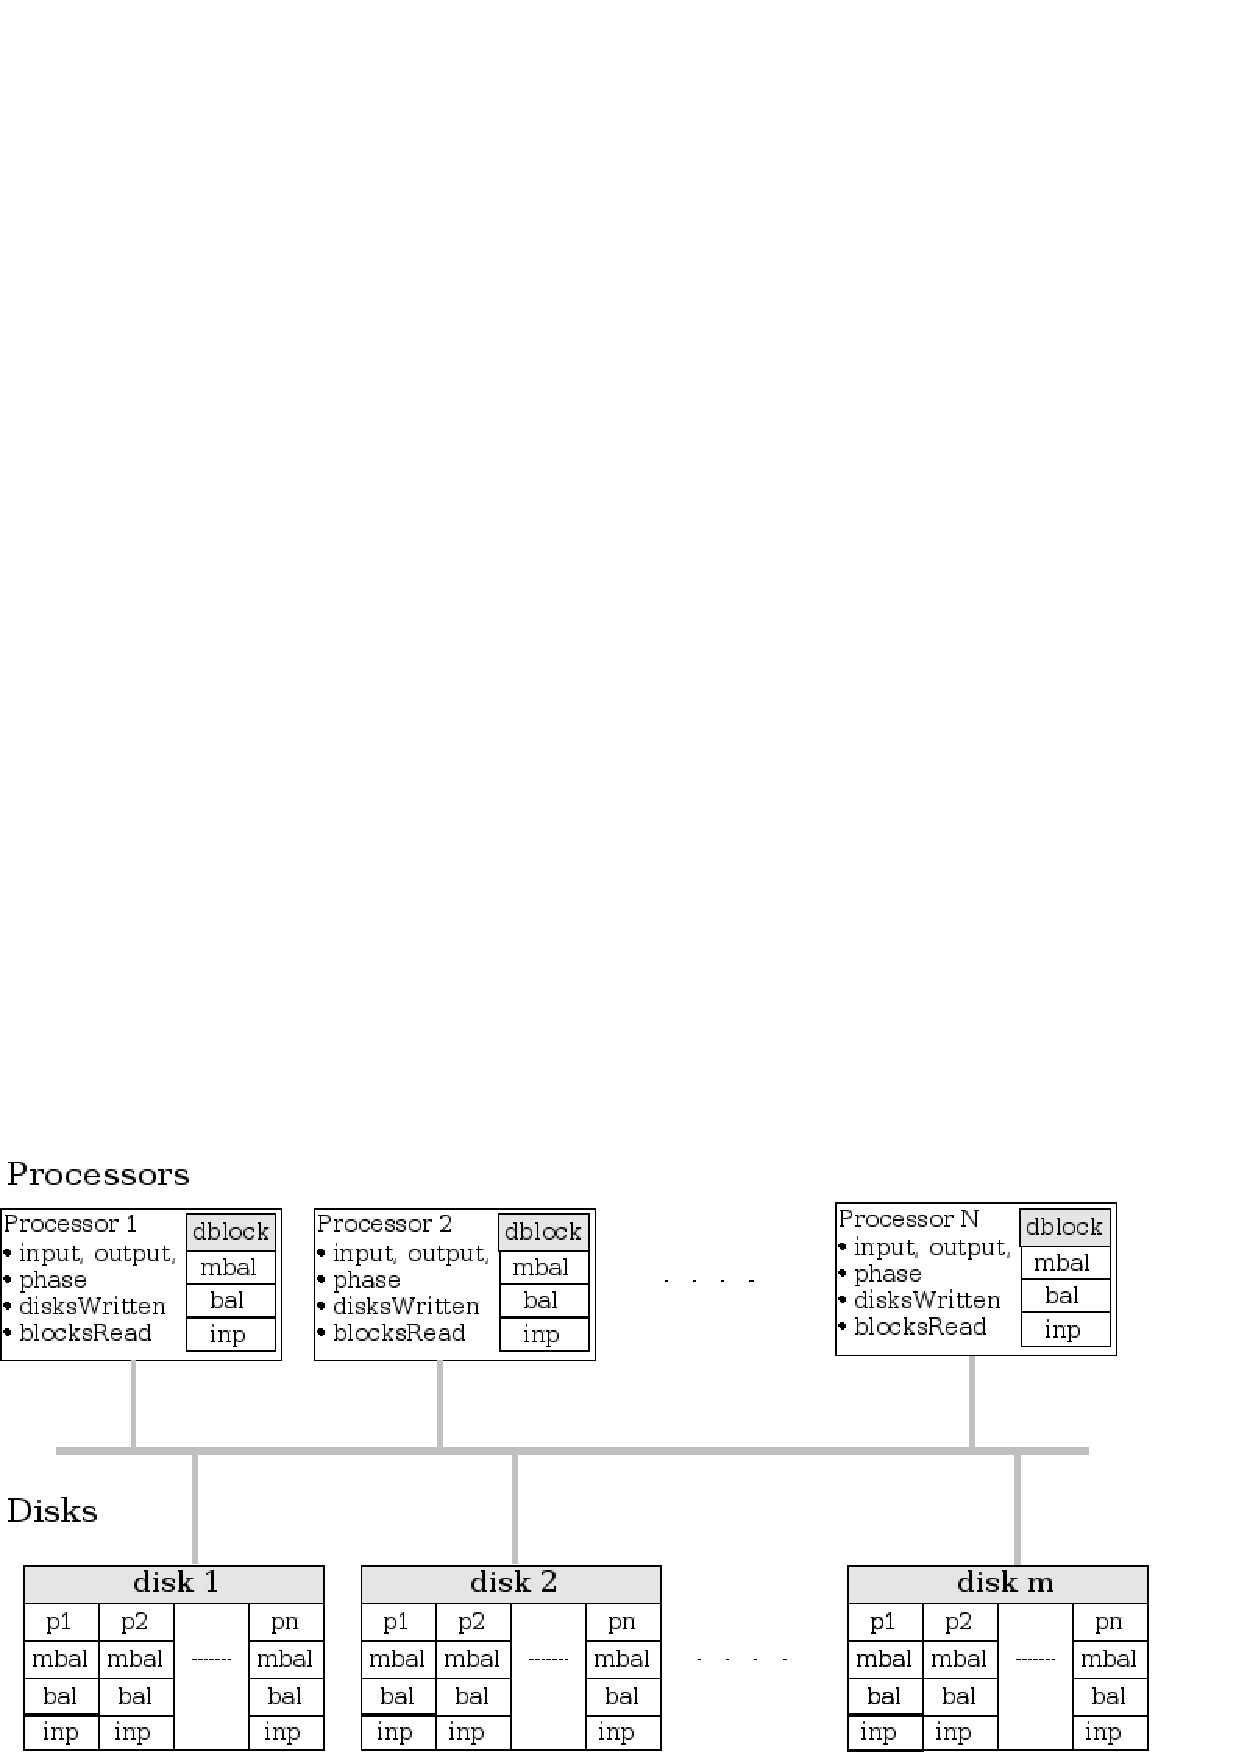
\includegraphics[%
  width=0.60\paperwidth,
  keepaspectratio]{DiskPaxos}
  \caption{\label{fig:proc_and_mem_blocks}A network of processors and
    disks.}
\end{figure}


For a complete description of the algorithm, see~\cite{Gafni00disk}.


\subsection{Disk Paxos and its TLA$^{+}$ Specification}

The specification of Disk Paxos is written in the TLA$^{+}$
specification language~\cite{LamportTLA:2002}. As it is usual with
TLA$^{+}$, the specification is organized into modules.

\tla The specification of consensus is given in module $Synod$, which
can be found in appendix \ref{ap:correctness}. In it there are only
two variables: $input$ and $output$. To formalize the property stating
that all processors should choose the same value and that this value
should have been an input of a processor, we need variables that
represent all past inputs and the value chosen as result.
Consequently, an $Inner$ submodule is introduced, which adds two
variables: $allInput$ and $chosen$. Our $Synod$ module will be obtained
by existentially quantifying these variables of the $Inner$ module.

The specification of the algorithm is given in the $HDiskSynod$
module.  Hence, what we are going to prove is that the (translation to
Isabelle/HOL of the) $Inner$ module is implied by the (translation to
Isabelle/HOL of the) algorithm module $HDiskSynod$.

More concretely we have that the specification of the algorithm is:

\[
HDiskSynodSpec == HInit /\ [] [HNext]_{\langle
  vars,chosen,allInput\rangle}\]

\noindent where $HInit$ describes the initial state of the algorithm
and $HNext$ is the action that models all of its state transitions.
The variable $vars$ is the tuple of all variables used in the
algorithm.

Analogously, we have the specification of the $Inner$ module:

\[
ISpec == IInit /\ [] [INext]_{\langle
  input,output,chosen,allInput\rangle}\]


We define $ivars=\langle input,output,chosen,allInput\rangle$. In
order to prove that $HDiskSynodSpec$ implies $ISpec$, we follow the
structure of the proof given by Gafni and Lamport. We must prove two
theorems:

\medskip{} $\THEOREM\, R1\qquad HInit => IInit$

$\THEOREM\, R2\qquad
HInit /\ [] [HNext]_{\langle
  vars,chosen,allInput\rangle} => [][INext]_{ivars}$
\medskip{}

The proof of $R1$ is trivial. For $R2$, we use TLA proof
rules~\cite{LamportTLA:2002} that show that to prove $R2$, it
suffices to find a state predicate $HInv$ for which we can prove:

\medskip{} 

$\THEOREM\, R2a\qquad HInit /\ [] [HNext]_{\;\langle
  vars,chosen,allInput\rangle} => [] HInv$

$\THEOREM\, R2b\qquad HInv /\ HInv' /\ HNext =>
INext \/ (\UNCHANGED ivars)$ 

\medskip

A predicate satisfying $HInv$ is said to be an invariant of
$HDiskSynodSpec$.  To prove $R2a$, we make $HInv$ strong enough to
satisfy:

\medskip

 $\THEOREM\, I1\qquad HInit => HInv$

$\THEOREM\, I2\qquad HInv /\ HNext => HInv'$
\medskip

Again, we have TLA proof rules that say that $I1$ and $I2$ imply
$R2a$. In summary, $R2b$, $I1$, and $I2$ together imply
$HDiskSynodSpec => ISpec$.

Finding a predicate $HInv$ that is strong enough can be rather
difficult.  Fortunately, Gafni and Lamport give this predicate. In
their paper, they present $HInv$ as a conjunction of 6 predicates
$HInv1,\ldots,HInv6$, where $HInv1$ is a simple {}``type invariant''
and the higher-numbered predicates add more and more information. The
proof is structured such that the preservation of $HInv\, i$ by the
algorithm's next-state relation relies on all $HInv\, j$ (for $j\leq
i$) being true in the state before the transition. In our proofs we
are going to use exactly the same tactic.

Before starting our proofs we have to translate all the specification
and theorems above into the formal language of Isabelle/HOL.

\notla

\section{Translating from TLA$^{+}$ to
  Isabelle/HOL\label{sec:Translating-from-TLA}}

The translation from TLA$^{+}$ to Isabelle/HOL is pretty
straightforward as Isabelle/HOL has equivalent counterparts for most
of the constructs in TLA$^{+}$ (some representative examples are shown
in table~\ref{tab:Examples-of-translations}).  Nevertheless, there are
some semantic discrepancies. In the following, we discuss these
differences, some of the options that one has when dealing with them,
and the reasons for our choices%
\footnote{There is no point in using the existing TLA encoding in
  Isabelle.  Since the encoding is also based on HOL and we only prove
  safety, we would have gained nothing.%
}.



%
\begin{table}
  \begin{tabular}{|c|c|}
    \hline 
    TLA$^{+}$&
    Isabelle/HOL\tabularnewline
    \hline
    \hline \tla 
    $\E d\in D\,:\, disk[d][q].bal=bk$&
    $\exists\ d\in D.\ bal(disk\ s\ d\ q)\ =\ bk$\tabularnewline
    \hline 
    $\CHOOSE x.P\, x$&
    $\varepsilon\ x.\ P\ x$\tabularnewline
    \hline 
    $phase'=[phase \EXCEPT ![p]=1]$&
    $phase\, s'=(phase\, s)(p:=1)$\tabularnewline
    \hline 
    $\UNION \{ \tla blocksOf(p)\,:\, p\,\in\, Proc\}$&
    $\mathit{UN}\ p.\ \mathit{blocksOf}\ s\ p$\tabularnewline
    \hline 
    $\UNCHANGED v$&
    $v\ s'=v\ s$\tabularnewline
    \hline
  \end{tabular}
\notla

  \caption{\label{tab:Examples-of-translations}Examples of TLA$^{+}$ formulas
    and their counterparts in Isabelle/HOL.}
\end{table}



\subsection{Typed vs. Untyped}

TLA$^{+}$ is an untyped formalism. However, TLA$^{+}$ specifications
usually have some type information, usually in the form of set membership
or set inclusion. When translating these specifications to Isabelle/HOL,
which is a typed formalism, one has to invent types that represent
these sets of values. This process is not automatic and requires some
thought to find the right abstractions. Furthermore, simple types
may not be expressive enough to represent exactly the set in the specification.
In some cases, these sets could be modelled by algebraic datatypes,
but this would make the specification more complex and less directly
related to the original one. In this work, we have chosen to stick
to simple types and add additional axioms to account for their lack
of expressiveness. 

%
\begin{figure}
TLA$^{+}$:

\medskip

\tla
$\CONSTANT Inputs$
\smallskip

$\begin{noj3}
NotAnInput & == & \CHOOSE c : c \not\in Inputs \\

\smallskip

DiskBlock & == & [ \begin{noj3}
                mbal & : & (\UNION {Ballot(p): p \in Proc})\cup\{ 0\}, \\
                bal  & : & (\UNION {Ballot(p): p \in Proc})\cup\{ 0\}, \\
                inp  & : & Inputs \cup \{NotAnInput\}]
                \end{noj3}
\end{noj3}$
\notla
\bigskip

Isabelle/HOL:

\medskip

\begin{isabellebody}
\isacommand{typedecl}\ InputsOrNi\isanewline
\isanewline
  \isacommand{consts}\isanewline
    \ \ Inputs\
    {\isacharcolon}{\isacharcolon}\ {\isachardoublequote}InputsOrNi\
    set{\isachardoublequote}\isanewline \ \ NotAnInput\
    {\isacharcolon}{\isacharcolon}\
    {\isachardoublequote}InputsOrNi{\isachardoublequote}\isanewline
    \isanewline 
  \isacommand{axioms}\isanewline \ \
    NotAnInput{\isacharcolon}\ {\isachardoublequote}NotAnInput\
    {\isasymnotin}\ Inputs{\isachardoublequote}\isanewline \ \
    InputsOrNi{\isacharcolon}\
    {\isachardoublequote}{\isacharparenleft}UNIV\
    {\isacharcolon}{\isacharcolon}\ InputsOrNi\ set{\isacharparenright}\
    {\isacharequal}\ Inputs\ {\isasymunion}\
    {\isacharbraceleft}NotAnInput{\isacharbraceright}{\isachardoublequote}\isanewline
  \isanewline
  \isacommand{record}\isanewline
    \ \ DiskBlock\ {\isacharequal}\ \isanewline
    \ \ \ \ mbal{\isacharcolon}{\isacharcolon}\ nat\isanewline
    \ \ \ \ bal\ {\isacharcolon}{\isacharcolon}\ nat\isanewline
    \ \ \ \ inp\ {\isacharcolon}{\isacharcolon}\ InputsOrNi\isanewline
\end{isabellebody}

\caption{\label{fig:Untyped-vs-Typed}Untyped TLA$^{+}$ vs. Typed Isabelle/HOL}
\end{figure}

\tla
For example, see figure~\ref{fig:Untyped-vs-Typed}. The type $InputsOrNi$
models the members of the set $Inputs$, and the element $NotAnInput$.
We record the fact that $NotAnInput$ is not in $Inputs$, with axiom
$NotAnInput$. Now, looking at the type of the $inp$ field of the
$DiskBlock$ record in the \notla TLA$^{+}$ \tla specification, we see that its
type should be $InputsOrNi$. However, this is not the same type as
$Inputs\cup\{ NotAnInput\}$, as nothing prevents the $InputsOrNi$
type from having more values. Consequently, we add the axiom $InputsOrNi$
to establish that the only values of this type are the ones in $Inputs$
and $NotAnInput$. 

\notla

This example shows the kind of difficulties that can arise when translating
from an untyped formalism to a typed one. Another solution to this
matter that is being currently investigated is the implementation
of native (untyped) support for TLA$^{+}$ in Isabelle, without relying
on HOL. 


\subsection{Primed Variables}

In TLA$^{+}$, to denote the value of a variable in the state resulting
from an action, there exists the concept of primed variables. In Isabelle/HOL,
there is no built-in notion of state, so we define the state as a record of
the variables involved. Instead of defining a {}``priming'' operator,
we just define actions as predicates that take any two states, intended
to be the previous state and the next state. In this way, $P\, s\, s'$
will be true iff executing an action $P$ in the $s$ state could
result in the $s'$ state. In figure~\ref{fig: primed_variables}
we can see how the action $Phase1or2Write$ is expressed in TLA$^{+}$
and in Isabelle/HOL.

%
\begin{figure}
TLA$^{+}$:

\medskip

\tla
$
Phase1or2Write(p,d) == \\ 
\s{1} \begin{conj}
    phase[p] \in \{1,2\} \\
    disk' = [disk \EXCEPT ![d][p]=dblock[p]] \\
    disksWritten' = [disksWritten \EXCEPT ![p]=@ \cup \{d\} ] \\
    \UNCHANGED \langle input,output,phase,dblock,blocksRead \rangle
  \end{conj}
$
\notla

\bigskip

Isabelle/HOL:

\begin{isabellebody}

\medskip

\ \ Phase{\isadigit{1}}or{\isadigit{2}}Write\ {\isacharcolon}{\isacharcolon}\ {\isachardoublequote}state\ {\isasymRightarrow}\ state\ {\isasymRightarrow}\ Proc\ {\isasymRightarrow}\ Disk\ {\isasymRightarrow}\ bool{\isachardoublequote}\isanewline
\ \ {\isachardoublequote}Phase{\isadigit{1}}or{\isadigit{2}}Write\ s\ s{\isacharprime}\ p\ d\ {\isasymequiv}\ \isanewline
\ \ \ \ \ phase\ s\ p\ {\isasymin}\ {\isacharbraceleft}{\isadigit{1}}{\isacharcomma}\ {\isadigit{2}}{\isacharbraceright}\isanewline
\ \ \ {\isasymand}\ disk\ s{\isacharprime}\ {\isacharequal}\ {\isacharparenleft}disk\ s{\isacharparenright}\ {\isacharparenleft}d\ {\isacharcolon}{\isacharequal}\ {\isacharparenleft}disk\ s\ d{\isacharparenright}\ {\isacharparenleft}p\ {\isacharcolon}{\isacharequal}\ dblock\ s\ p{\isacharparenright}{\isacharparenright}\ \isanewline
\ \ \ {\isasymand}\ disksWritten\ s{\isacharprime}\ {\isacharequal}\ {\isacharparenleft}disksWritten\ s{\isacharparenright}\ {\isacharparenleft}p{\isacharcolon}{\isacharequal}\ {\isacharparenleft}disksWritten\ s\ p{\isacharparenright}\ {\isasymunion}\ {\isacharbraceleft}d{\isacharbraceright}{\isacharparenright}\isanewline
\ \ \ {\isasymand}\ inpt\ s{\isacharprime}\ {\isacharequal}\ inpt\ s\ {\isasymand}\ outpt\ s{\isacharprime}{\isacharequal}\ outpt\ s\isanewline
\ \ \ {\isasymand}\ phase\ s{\isacharprime}\ {\isacharequal}\ phase\ s\ {\isasymand}\ dblock\ s{\isacharprime}\ {\isacharequal}\ dblock\ s\isanewline
\ \ \ {\isasymand}\ blocksRead\ s{\isacharprime}{\isacharequal}\ blocksRead\ s{\isachardoublequote}\isanewline
\end{isabellebody}

\caption{\label{fig: primed_variables}Translation of an action}
\end{figure}



\subsection{Restructuring the specification}

There are some minor changes that can be made to specifications to
make the proofs in Isabelle easier. 

One such change is the elimination of \textsc{let} constructs by making
them global definitions. This has two benefits, as it makes it possible
to:

\begin{itemize}
\item Formulate lemmas that use these definitions.
\item Selectively unfold these definitions in proofs, instead of adding
\mbox{$Let\isacharunderscore def$} to Isabelle's simplifier, which unfolds all {}``let''
constructs.
\end{itemize}
Another change that makes proofs easier is to break down actions into
simpler actions (e.g. giving separate definitions for subactions corresponding
to disjuncts). By making actions smaller, Isabelle has to deal with
smaller formulas when we feed the prover with such an action.

\tla
For example, $Phase1or2Read$ is mainly a big if-then-else. We break
it down into two simpler actions: \[
Phase1or2Read == Phase1or2ReadThen \/ Phase1or2ReadElse\]


\noindent In $Phase1or2ReadThen$ the condition of the if-then-else
is present as a state formula (i.e. it is an enabling condition) while
in $Phase1or2ReadElse$ we add the negation of this condition.

Another example is $HInv2$, which we break down into:

\[
HInv2 == Inv2a /\ Inv2b /\ Inv2c\]

\notla

Not only we break it down into three conjuncts but, since these
conjuncts are quantifications over some predicate, we give a separate
definition for this predicate. For example for $Inv2a$, and after
translating to Isabelle/HOL, instead of writing:

\medskip
\begin{isabellebody}
Inv{\isadigit{2}}a\ s\ {\isasymequiv}\
  {\isasymforall}p{\isachardot}\
{\isasymforall}bk\ {\isasymin}\ blocksOf\ s\
  p{\isachardot}\ \ldots 
\end{isabellebody}

\smallskip
\noindent we write:
\medskip

\begin{isabellebody}
  \ \
  Inv{\isadigit{2}}a{\isacharunderscore}innermost\
  {\isacharcolon}{\isacharcolon}\ {\isachardoublequote}state\
  {\isasymRightarrow}\ Proc\ {\isasymRightarrow}\ DiskBlock\
  {\isasymRightarrow}\ bool{\isachardoublequote}\isanewline \ \
  {\isachardoublequote}Inv{\isadigit{2}}a{\isacharunderscore}innermost\
  s\ p\ bk\ {\isasymequiv}\ \ldots\isanewline
  \isanewline \ \ Inv{\isadigit{2}}a{\isacharunderscore}inner\
  {\isacharcolon}{\isacharcolon}\ {\isachardoublequote}state\
  {\isasymRightarrow}\ Proc\ {\isasymRightarrow}\
  bool{\isachardoublequote}\isanewline \ \
  {\isachardoublequote}Inv{\isadigit{2}}a{\isacharunderscore}inner\ s\
  p\ {\isasymequiv}\ {\isasymforall}bk\ {\isasymin}\ blocksOf\ s\
  p{\isachardot}\ Inv{\isadigit{2}}a{\isacharunderscore}innermost\ \
  s\ p\ bk{\isachardoublequote}\isanewline \isanewline \ \
  Inv{\isadigit{2}}a\ {\isacharcolon}{\isacharcolon}\
  {\isachardoublequote}state\ {\isasymRightarrow}\
  bool{\isachardoublequote}\isanewline \ \
  {\isachardoublequote}Inv{\isadigit{2}}a\ s\ {\isasymequiv}\
  {\isasymforall}p{\isachardot}\
  Inv{\isadigit{2}}a{\isacharunderscore}inner\ s\
  p{\isachardoublequote}\isanewline
\end{isabellebody}

Now we can express that we want to obtain the fact

\medskip

\begin{isabellebody}
 \ \ \ \ \ \ 
 Inv{\isadigit{2}}a{\isacharunderscore}innermost\ s\ q\ (dblock\ s\ q)
\end{isabellebody}

\medskip

\noindent explicitly stating that we are interested in predicate
$Inv2a$, but only for some process $q$ and block $(dblock\ s\ q)$.



\section{Structure of the Correctness Proof}
\label{sec:Structure-of-the}

In~\cite{Gafni00disk}, a specification of correctness and a
specification of the algorithm are given. Then, it is proved that the
specification of the algorithm implies the specification of
correctness. We will do the same for the translated specifications,
maintaining the names of theorems and lemmas. It should be noted that
only safety properties are given and proved.


\subsection{Going from Informal Proofs to Formal Proofs}
\tla
There are informal proofs for invariants
$HInv3$-$HInv6$ and for theorem $R2b$
in~\cite{Gafni00disk}. These informal proofs are written in the
structured-proof style that Lamport advocates~\cite{Lamport95how}, and
are rigorous and quite detailed. We based our formal proofs on these
informal proofs, but in many cases a higher level of detail was
needed. In some cases, the steps where too big for Isabelle to solve
them automatically, and intermediate steps had to be proved first; in
other cases, some of the facts relevant to the proofs were omitted in
the informal proofs.

As an example of these omissions, the invariant should state that the
set $allRdBlks$ is finite. This is needed to choose a block with a
maximum ballot number in action $EndPhase1$. Interestingly, this
omission cannot be detected with finite-state model checking. As
another example, it was omitted that it is necessary to assume that
$HInv4$ and $HInv5$ hold in the previous state to prove lemma $I2f$.

Although our proofs were based on the informal ones, the high-level
structure was often different. When proving that a predicate $I$ was
an invariant of $Next$, we preferred proving the invariance of $I$ for
each action, rather than a big theorem proving the invariance of $I$
for the $Next$ action.  As a consequence, a proof for some actions was
often similar to the proof of some other action. For example, the
proof of the invariance of $HInv3$ for the $EndPhase0$ and $Fail$
actions is almost the same. This means we could have made only one
proof for the two actions, shortening the length of the complete
proof.  Nevertheless, proving each action separately could be tackled
more easily by Isabelle, as it had fewer facts to deal with, and
proving a new lemma was often a simple matter of copy, paste and
renaming of definitions. Once the invariance of a given predicate has
been proved for each simple action, proving it for the $Next$ action is
easy since the $Next$ action is a disjunction of all
actions.

The informal proofs start working with $Next$, and then do a case
split in which each case implies some action. The structure of the
formal proof was copied from the informal one, in the parts where the
latter focused on a particular action, This structure could be easily
maintained since we used Isabelle's Isar proof
language~\cite{Wenzel02isabelleisar,Nipkow-TYPES02}, a language for
writing human-readable structured proofs.

Lamport's use of a hierarchical scheme for naming subformulas of a
formula would have been very useful, as we have to repeatedly extract
subfacts from facts. These proofs were always solved automatically by
the auto Isabelle tactic, but made the proofs longer and harder to
understand. Automatic naming of subformulas of Isabelle definitions
would be a very practical feature.

\notla

\section{Conclusion}\label{sec:Conclusion}

We formally verified the correctness of the Disk Paxos specification
in Isabelle/HOL. We found some omissions in the informal proofs, including
one that could not have been detected with finite-state model checking,
but no outright errors. This formal proof gives us a greater confidence
in the correctness of the algorithm. 

This work was done in little more than two months, including learning
Isabelle from scratch. Consequently, this work can be taken as evidence
that formal verification of fault-tolerant distributed algorithms
may be feasible for software verification in an industrial context.

Isabelle proved to be a very helpful tool for this kind of verification,
although it would have been useful to have Lamport's naming of subfacts
to make proofs shorter and easier to write.

\bibliographystyle{alpha}
\bibliography{root}



%%% Local Variables: 
%%% mode: latex
%%% TeX-master: "root"
%%% End: 


%\newpage

\appendix

\section{TLA$^{+}$ correctness specification}
\label{ap:correctness}

\tla
\begin{module}{Synod}
\EXTENDS Naturals

%\textsc{extends}\ Naturals

\CONSTANT N, Inputs

\ASSUME $(N \in Nat) /\ (N>0)$

$Proc == 1 .. N$

$NotAnInput == \CHOOSE c : c\not\in Inputs$

$\VARIABLES inputs, output$

\vs{1.2}

\begin{submodule}{Inner}
$\VARIABLES allInput, chosen$

\midbar

\vs{1}

$IInit ==$ 
  \begin{conj} 
    input  \in [Proc \rightarrow Inputs] \\
    output  = [p \in Proc \mapsto NotAnInput]\\
    chosen  = NotAnInput \\
    allInput  = {input[p]: p \in Proc}
  \end{conj}

\vs{1.2}

$IChoose(p) == $
\s{1.2} \begin{conj}
    output[p] = NotAnInput \\
    \begin{noj}
      \IF{chosen = NotAnInput} \\
        \THEN ip \in allInput : 
          \begin{conj}
            chosen' = ip \\
            output' = [output \EXCEPT ![p] = ip]
          \end{conj}
        \ELSE \begin{conj}
                 output' = [output \EXCEPT ![p]=chosen] \\
                 \UNCHANGED chosen
               \end{conj}
      \FI
    \end{noj} \\
    \UNCHANGED \langle input, allInput \rangle 
  \end{conj}
    
\vs{1.2}

$IFail(p) ==$
  \begin{conj}
    output' = [output \EXCEPT ![p]=NotAnInput] \\
    \E ip \in Inputs : \begin{conj}
                         input' = [input \EXCEPT ![p] = ip]\\
                         allInput' = allInput \cup \{ip\}
                       \end{conj}
  \end{conj}

\vs{1.2}

$INext == \E p \in Proc : IChoose(p) \/ IFail(p)$

$ISpec == IInit /\ [] [INext]_{\langle input,output,chosen,allInput \rangle}$

\end{submodule} 

\vs{1.2}

$IS(chosen,allInput) == \INSTANCE Inner$

$SynodSpec == \EE chosen, allInput : IS(chosen, allInput)!ISpec$
\end{module}

%%% Local Variables: 
%%% mode: latex
%%% TeX-master: "root"
%%% End: 

\notla
\parindent 0pt\parskip 0.5ex

% include generated text of all theories
\input{session}

\end{document}
